% \pagebreak[4]
% \hspace*{1cm}
% \pagebreak[4]
% \hspace*{1cm}
% \pagebreak[4]

\chapter{Tối ưu hóa hiệu quả tính toán trong Word2Vec}
\ifpdf
    \graphicspath{{Chapter1/Chapter1Figs/PNG/}{Chapter1/Chapter1Figs/PDF/}{Chapter1/Chapter1Figs/}}
\else
    \graphicspath{{Chapter1/Chapter1Figs/EPS/}{Chapter1/Chapter1Figs/}}
\fi
Như đã nói, tất cả các model (“bigarm”, CBOW, skip-gram) chúng ta tìm hiểu ở bài báo cáo trước đều là dạng nguyên thủy của chúng, hoàn toàn không được áp dụng các biện pháp tối ưu hóa hiệu quả.

Trong toàn bộ các model này, mỗi từ trong tập từ vựng luôn tồn tại 2 vector là vector đầu vào $v_m$ và vector đầu ra $v'_m$. Học vector đầu  vào thì tốn ít chi phí, nhưng học vector đầu ra thì rất tốn chi phỉ xử lý. Từ các phương trình cập nhật cơ bản được nêu ở các mục trước, ta thấy rằng để cập nhật $v'_m$ cho mỗi một training instance, ta bắt buộc phải duyệt loại toàn bộ các từ $w_j$ trong tập từ vựng và tính toán lại các thành phần : mạng đầu vào $u_j$, dự đoán xác suất $y_j$ (hoặc $y_{c,j}$ với skip-gram) , giá trị dự đoán lỗi $e_j$ ($EI_j$  với skip-gram) và cuối cùng sử dụng giá trị dự đoán lỗi để cập nhật vector đầu ra $v'_j$.

Thực hiện những tính toán như vậy với toàn bộ các từ trong từ training instance là rất tốn chi phí cũng như tài nguyên, khiến cho các model này trở thành bất khả thi khi mở rộng cho việc training liên tục. Để giải quyết vấn đề này, một phương án đưa ra là giới hạn số lượng vector đầu ra bắt buộc phải cập nhật trên mỗi training instance.

Một phương pháp tiếp cận khá nhẹ nhàng là cho phương án trên là “soft-max có thứ bậc”  (hierarchial soft-max) ; ngoài ra còn có một phương pháp khác thông qua việc lấy mẫu, cách này sẽ được trình bày ở mục sau. \\[0.5cm]
\section{Hierarchial soft-max}
Hierarchial soft-max là một trong những phương pháp hiệu của của tính toán soft-max. Mô hình này sử dụng một cây nhị phân để đại diện tất cả các từ trong tập từ vựng.  V từ bắt buộc phải là nút lá của cây. Có thể chứng minh là có V-1 nút trong. Với mỗi một nút lá, tồn tại một đường duy nhất từ gốc đến nút này và đường đi này được dùng để ước tính xác suất của từ được đại diện bởi nút lá.
\begin{figure}[!htbp]
  \begin{center}
    %\leavevmode
    \ifpdf
      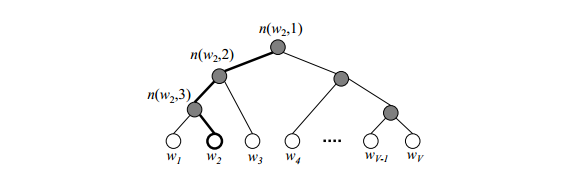
\includegraphics[scale=1.0]{HierarchialSoftmax}
    \else
      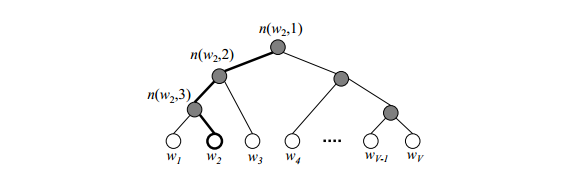
\includegraphics[scale=1.0]{HierarchialSoftmax}
    \fi
    \caption{Hierarchial Softmax}
    \label{HierarchialSoftmax}
  \end{center}
\end{figure}

Như hình trên, mỗi một nút trắng là là một từ trong tập từ vựng, còn các nút xám là các nút trong. Đường tô đậm là đường đi từ gốc đến nút lá đại diên cho từ $w_2$. Chiều dài của đường đi $L(w_2)=4$. $n(w,j)$ là nút thứ $j$ trên đường đi từ gốc đến từ $w$.

Trong mô hình hierarchical soft-max, không có vector đầu ra đại diện cho từ. thay vào đó mỗi 1 nút trong đại sẽ có 1 vector đầu ra $\textbf{v'}_{n(w,j)}$ và xác suất của một từ trở thành từ đầu ra được tính theo công thức:
\begin{eqnarray}
p(w=w_O)= \prod^{L(w)-1}_{j=1}\sigma\left( \left[  \left[ n(w,j+1)=ch(n(w,j)) \right]  \right] . {\textbf{v'}_{n(w,j)}}^{T} \textbf{h} \right) 
\end{eqnarray}

Với $ch(n)$ là con trái của $n$. $\textbf{v}'_{n(w,j)}$ là vector đại diện cho node $n(w,j)$. $h$ là giá trị đầu ra của layer ẩn ($\textbf{h}=w_j$ với skip-gram và bằng $\frac{1}{C}$ $\sum^{C}_{c=1} v_{w_c}$ với CBOW). $[[x]]$ là một hàm đặc biệt trả về giá trị $1$ nếu $x$ đúng và $-1$ trong trường hợp còn lại.

Để có cái nhìn trực quan hơn về phương trình trên, chúng ta sẽ tìm hiểu ví dụ một cách chi tiết hơn. Nhìn vào hình {\ref{HierarchialSoftmax}}, giả sử như ta muốn tính toán xác suất $w_2$ là từ đầu ra, ta định nghĩa xác xuất suất này là xác suất xác suất của một đường đi ngẫu nhiên bắt đầu từ gốc đến node lá trong câu hỏi. Với mỗi một node trong (tính cả gốc) ta cần chỉ định xác suất của việc đi sang trái hay đi sang bên phải \footnote{Một cây nhị phân bất kỳ thì nút trong ko phải lúc nào cũng có cả 2 con trái, phải. Tuy nhiên cây nhị phân Huffman luôn tồn tại cả 2 con trái, phải. Mặc dù có thể sử dụng nhiều loại cây khác nhau cho  hierarchical softmax nhưng trong word2vec ta sử dụng cây Huffman để tăng tốc độ training}.

Ta định nghĩa xác suất sang trái của node n là:
\begin{eqnarray}
p(n,left)= \sigma\left( \textbf{v}'^{T}_{n} . \textbf{h} \right) 
\end{eqnarray}
Xác suất này được xác định vector đại diện của node trong, và giá giá trị đầu ra của layer ẩn (được xác định bằng vector đại diện của từ đầu vào).

Tương tự ta định nghĩa xác suất sang trái của node n là:
\begin{eqnarray}
p(n,right)= 1 - p(n,left) = \sigma\left( -\textbf{v}'^{T}_{n} . \textbf{h}\right) 
\end{eqnarray}
Nhìn vào đường đi từ gốc đến $w_2$ trong hình \ref{HierarchialSoftmax}, Ta có thể tính toán được xác suất của mà $w_2$ sẽ là từ đầu ra:

\begin{eqnarray}
\begin{split}
p(w=w_O) &=p\left( n(w_2,1),left)\right) .p\left( n(w_2,2),left)\right) .p\left( n(w_2,3),right)\right) \\
&=\sigma\left( {\textbf{v}'_{n(w_2,1)}}^{T} \textbf{h} \right) . \sigma\left( {\textbf{v}'_{n(w_2,2)}}^{T} \textbf{h} \right) . \sigma\left( {-\textbf{v}'_{n(w_2,3)}}^{T} \textbf{h} \right)
\end{split}
\end{eqnarray}

%\begin{equation}

 % \begin{array}{l l}
 %   p(w=w_O) & =p\left( n(w_2,1),left)\right) .p\left( n(w_2,2),left)\right) .p\left( %n(w_2,3),right)\right)  \\
 %    & = \sigma\left( {v'_{n(w_2,1)}}^{T} h \right) . \sigma\left( %{\textbf{v}'_{n(w_2,2)}}^{T} h \right) . \sigma\left( {-\textbf{v}'_{n(w_2,3)}}^{T} h \right)
 % \end{array}

%\end{equation}


Nó hoàn toàn giống với công thức (37) đã nêu ra ở báo cáo GR1 và dễ chứng minh rằng hierarchical softmax là một đa thức phân phối đều trên toàn tập $V$:
\begin{eqnarray}
\sum^{V}_{i=1} p(w_i=w_O) =1
\end{eqnarray}

Giờ ta lấy được thông số phương trình cập nhật cho vector đại diện của node trong. Để đơn giản, ta bắt đầu từ mô hình context một từ sau đó đến các mô hình CBOW và skip-gram. 

Để tiện trong việc trình bày ta viết tắt một số giá trị đã xuất hiện ở trên:
\begin{equation}
\left[ \left[ . \right] \right] := \left[  \left[ n(w,j+1)=ch(n(w,j)) \right]  \right]
\end{equation}
\begin{equation}
\textbf{v}'_j := \textbf{v}'_{n_(w,j)}
\end{equation}

Với mỗi một Instance tập huấn, hàm lỗi được định nghĩa bằng:
\begin{equation}
E = - \log{p\left( w = w_O|w_I \right)} = -\sum^{L(w)-1}_{j=1}\sigma\left( \left[ \left[ . \right] \right] \textbf{v}'^{T}_{j} \textbf{h} \right) 
\end{equation}

Ta tính đạo hàm của $E$ theo $\textbf{v}'_j\textbf{h}$ thu được:
\begin{equation}
\begin{split}
\dfrac{\partial E}{\partial \textbf{v}'_j\textbf{h}} &= \left( \sigma{([[.]] \textbf{v}'^{T}_{j} \textbf{h})}  \right) - 1 \\
&= \left\{ \begin{array}{l l}
    \quad \sigma{ \left( \textbf{v}'^{T}_{j} \textbf{h}\right) } - 1 &  ([[.]] = 1)\\
    \quad \sigma{ \left( \textbf{v}'^{T}_{j} \textbf{h}\right) } &  ([[.]] = -1) \\
  \end{array} \right. \\
&= \sigma{ \left( \textbf{v}'^{T}_{j} \textbf{h}\right) } - t_j\\
\end{split}
\end{equation}
Với $t_j=1$ với $[[.]] = 1 $ và $t_j=0$ trong trường hợp còn lại.

Tiếp theo ta tính đạo hàm của $E$ theo vector đại diện của node trong $n(w,j)$ thu được:
\begin{equation}
\dfrac{\partial{E}}{\partial{\textbf{v}'_{j}}} = \dfrac{\partial{E}}{\partial{\textbf{v}'_{j} \textbf{h}}} . \dfrac{\partial{\textbf{v}'_{j} \textbf{h}}}{\partial{\textbf{v}'_{j}}} = \left( \sigma  \left( \textbf{v}'^{T}_{j} \textbf{h}\right) - t_j \right) . \textbf{h}
\end{equation}

Kết quả này sẽ được sử dụng trong phương trình cập nhật dưới đây với $j=1,2 ,…,L(w)-1$

\begin{equation}
{\textbf{v}'_{j}}^{(new)} = {\textbf{v}'_{j}}^{(old)} - \eta \left( \sigma \left( {\textbf{v}'_{j}}^{T} \textbf{h}\right) - t_j \right) . \textbf{h}
\end{equation}

Có thể hiểu rằng $\sigma \left( {\textbf{v}'_{j}}^{T} \textbf{h} \right) - t_j $ như là giá trị dự đoán lỗi của node trong $n(w,j)$.  Nhiệm vụ của mỗi node trong là dự đoán xem nên rẽ sang con trái hay con phải trong đường đi. $t_j=1$ nghĩa là lựa chọn rẽ sang con trái, và bằng 0 nếu lựa chọn rẽ sang con phải. $\sigma \left( {\textbf{v}'_{j}}^{T} \textbf{h} \right) - t_j $ được gọi là kết quả dự đoán. Với mỗi 1 trainning instance, nếu như dự đoán của node trong rất gần với thực tế. thì vector đại diện $\textbf{v}'_{j}$ sẽ dịch chuyển ít hơn và ngược lại nếu dự đoán khác thực tế quá nhiều thì vector đại diện $ \textbf{v}'_{j} $ sẽ phải dịch chuyển nhiều hơn để giảm giá trị dự đoán lỗi. (có thể gần lại hoặc ra xa $ \textbf{h} $ ).  Phương trình cập nhật này có thể được sử dụng cho cả CBOW và skip-gram. Tuy nhiên khi sử dụng cho mô hình skip-gram ta cần lặp lại quá trình cập nhật này cho mỗi bộ $C$ từ trong context đầu ra.

Nhằm truyền ngược lại lỗi để học trọng số trong quá trình “input->hidden” ta tính đạo hàm của E theo đầu ra của của layer ẩn :
\begin{equation}
\begin{split}
\dfrac{\partial{E}}{\partial{\textbf{h}}} &= \sum^{L(w)-1}_{j=1} \dfrac {\partial{E}}{\partial{\textbf{v}'_{j} \textbf{h}}} . \dfrac{\partial{\textbf{v}'_{j} \textbf{h}}}{\partial{ \textbf{h}}}\\
&= \sum^{L(w)-1}_{j=1} \left( \sigma  \left( \textbf{v}'^{T}_{j} \textbf{h}\right) - t_j \right) . \textbf{v}'_{j} \\
&:=EH
\end{split}
\end{equation}

Ta có thể dùng phương trình trên để trực tiếp thế vào các phương trình cập nhật cho vector đầu vào trong mô hình CBOW hay mô hình skip-gram. Khi áp dụng vào skip-gram thì ta cần tính tổng của EH của từng word trong context rồi mới áp dụng.

\section{Mẫu tiêu cực}

Ý tưởng của biện pháp mẫu tiêu cực (negative sampling) trực tiếp hơn hierarchical softmax: để ứng phó với việc phải có quá nhiều nodes phải tính toán với mỗi một vòng lặp, ta chỉ lấy mẫu một vài nodes mà ta tính toán điểm số.  

Hiển nhiên ta cần phải giữ các từ đầu ra trong thực tế là các mẫu tích cực và cần phải lấy mẫu thêm các ví dụ tiêu cực ( vì thế mà phương pháp này được gọi là mẫu tiêu cực). 

Trong word2vec \cite{DBLP:conf/nips/MikolovSCCD13} thay vì sử dụng cách thức chuẩn của phương pháp mẫu tiêu cực, tác giả đã sử dụng một cách hàm training giản lược với mỗi instance từ đầu ra như sau:
\begin{equation}
E= - \log{ \sigma \left( {\textbf{v}'_{w_O}}^{T} \textbf{h}\right)} - \sum^{L(w)-1}_{j=1} \log{ \sigma \left( {\textbf{v}'_{w_i}}^{T} \textbf{h}\right)}
\end{equation}

với $ \left\lbrace  w_i | i=1,2,…K \right\rbrace $được lấy mẫu từ phân tán nhiễu , $h$ là giá trị đầu ra của layer ẩn. Trong mô hình skip gram thì $h= \textbf{v}_{w_I}$ còn trong mô hình CBOW $h=\dfrac{1}{C} \sum^{C}_{c=1} \textbf{v}_{w_c}$;  $\textbf{v}_w$ là vector đầu vào của từ $w$, được lấy từ một hàng của ma trận trọng số input  $ \rightarrow $ hidden, ; $\textbf{v}'_w$ là vector đầu ra, được lấy từ một cột của ma trận trọng số hidden $ \rightarrow $ output. Mỗi từ đều có 2 vector đại diện như vậy. 

Ta tính đạo hàm của $E$ theo ${\textbf{v}'_{w_j}}^{T} \textbf{h}$ :
\begin{equation}
\begin{split}
\dfrac{\partial{E}}{\partial{{\textbf{v}'_{w_j}}^{T} \textbf{h}}} &= \left\{ \begin{array}{l l}
    \quad \sigma{ \left( {\textbf{v}'_{w_i}}^{T} \textbf{h}\right) } - 1 &  (w_j=w_O) \\
    \quad \sigma{ \left( {\textbf{v}'_{w_i}}^{T} \textbf{h}\right) } &  w_j \in \left\lbrace w_i|i=1,2,...,K \right\rbrace \\
  \end{array} \right. \\
  &= \sigma \left( {\textbf{v}'_{w_i}}^{T} \textbf{h}\right) - t_j
\end{split}
\end{equation}
với $t_j$ là “nhãn” của từ $w_j$. $t=1$ khi $w_j$ là mẫu tích cực, và bằng 0 trong trường hợp ngược lại. 
	Tiếp theo ta tính dạo hàm của E theo vector đầu ra $\textbf{v}'_{w_j}$ :
\begin{equation}
\dfrac{\partial{E}}{\partial{\textbf{v}'_{w_j}}} = \dfrac{\partial{E}}{\partial{{\textbf{v}'_{w_j}}^{T} \textbf{h}}} . \dfrac{\partial{{\textbf{v}'_{w_j}}^{T} \textbf{h}}}{\partial{\textbf{v}'_{w_j}}} = \left( \sigma \left( \textbf{v}'^{T}_{j} \textbf{h}\right) - t_j \right) . \textbf{h}
\end{equation}
và sử dụng kết quả này trong việc cập nhật vector đầu ra :
\begin{equation}
{\textbf{v}'_{w_j}}^{(new)} = {\textbf{v}'_{w_j}}^{(old)} - \eta \left( \sigma \left( {\textbf{v}'_{w_j}}^{T} \textbf{h}\right) - t_j \right) . \textbf{h}
\end{equation}

với $w_j  \in \left\lbrace w_O \right\rbrace \cup \left\lbrace w_i \sim P_n(w)|i=1,2,…K \right\rbrace $

Rõ ràng  số phép tính toán ở đây đã ít hơn so với công thức đã trình bày ở bài báo cáo trước khi ta không còn phải chạy trên toàn bộ tập từ. Phương trình cập nhật ở trên có thể dùng cho cả CBOW và skip-gram. 
 
 Để truyền ngược lỗi input $\rightarrow$ hidden và thông qua đó để cập nhật vector đầu vào của từ ta cần tính đạp hàm của $E$ theo đầu ra $\textbf{h}$ của layer ẩn. 
\begin{equation}
\dfrac{ \partial{E} }{\partial{\textbf{h}}} =\dfrac {\partial{E}}{\partial{ {\textbf{v}'_{w_j}}^{T} \textbf{h}}} . \dfrac{\partial{{\textbf{v}'_{w_j}}^{T} \textbf{h}}}{\partial{ \textbf{h}}} =\left( \sigma  \left( {\textbf{v}'_{w_j}}^{T} \textbf{h}\right) - t_j \right) . \textbf{v}'_{w_j} :=EH
\end{equation}
 
EH sẽ được sử dụng trong phương trình cập nhật cho vector đầu vào của CBOW hay mô hình skip-gram. Khi áp dụng với skip-gram, ta cần tính tổng toàn bộ EH với mọi context sau đó dùng tổng này vào phương trình cập nhật.